\section{Extração e armanezamento de notícias}
As notícias são extraídas de várias fontes jornalísticas e são introduzidas numa plataforma de indexação chamada \textit{whoosh}. O \textit{whoosh} compila as notícias utilizando o algoritmo de classificação \textit{BM25}. Posteriormente, são armazenadas numa colecção de notícias na nossa base de dados não relacional \textit{MongoDB}. Para aumentar a velocidade da extracção, os pedidos às páginas \textit{web} são separados em \textit{threads} com o objectivo de conseguirmos um maior \textit{throughput} visto que a comunicação pela internet é o maior \textit{bottleneck} da aplicação.

Na nossa aplicação o \textit{feedparser}, acede a um conjunto de \textit{links} RSS do qual extrai os endereços das notícias que são acedidos paralelamente. Cada página é analisado com o \textit{beautiful soup} sendo extraídos unicamente o título e o corpo do artigo. Para isto, foram criados três \textit{parsers} que lidam com a estrutura da páginas de maneira diferente dependendo do site da notícia.

As notícias são armazenadas na base de dados com o objectivo de evitar colisões, ou seja, caso uma notícia já tenha sido processada anteriormente, não é indexada novamente. Além disso, o \textit{whoosh} apresenta os resultados com os \textit{links} das notícias, para que depois os elementos de cada notícia possam ser acedidos a partir da base de dados, utilizando o \textit{link} como chave. Por fim, faz-se a extração e armazenamento das entidades. Este último tópico é explicado em detalhe nas secções seguintes.

Na figura seguinte, apresentamos o fluxo de execução descrito anteriormente.

\begin{figure}[htbp]
  \centering
    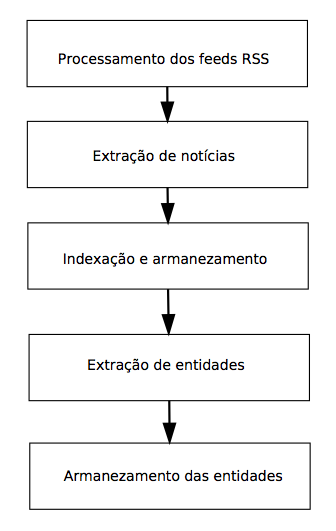
\includegraphics[width=0.4\textwidth]{images/fluxo.png}
    \caption{Fluxo de execução}
\end{figure}

